\chapter{Предметная область} \label{chapt1}
% % %todo убрать висящие строки
Данные о плотности грунта служат основанием для оценки залежей полезных ископаемых 
и принятия решения о начале геологоразведки перспективных районов. На основании  информации о плотности грунта 
определяются порядок, объемы и состав проектных работ при подготовке к строительству зданий и дорог, делаются заключения о безопасности проводимых 
строительных работ, качестве их выполнения и возможности ввода в эксплуатацию возведенных сооружений. При подготовке ряда объектов 
(фундаментов зданий, шоссе, железнодорожных насыпей) проводятся 
работы по уплотнению грунта, для определения объема которых необходимы измеренные и требуемые значения показателей плотности сухого грунта.
Мониторинг плотности грунта позволяет контролировать и упреждать возникновение аварийных ситуаций при эксплуатации уже возведенных объектов, 
в частности, таких, как высотные здания, мосты, железнодорожные насыпи, линии метро, шахты, аэродромы.


\section{Методы измерения плотности грунта в геологии} \label{sect1_1}

Плотность грунта измеряется либо контактными методами через непосредственный замер плотности образцов, 
либо бесконтактными, либо радиационными методами. 
В обоих случаях предполагается бурение исследуемого грунта. 

\subsection{Контактные методы}\label{subsect1_1_1}

В ГОСТ-5180-84. ``Грунты. Методы лабораторного определения физических характеристик`` описаны следующие 
методы измерения плотности грунта --- режущим кольцом, взвешивание в воде парафинированных образцов, и 
взвешивание мерзлых пород в нейтральных жидкостях . В зависимости от типа грунта, его сыпучести и содержания воды,
выбирается тот или иной метод. Масса образца грунта оставляет от пары сотен грамм до нескольких килограмм. При этом, чтобы получить 
распределение плотности грунта проводится ряд параллельных замеров. Значение характеристик вычисляют как 
среднее арифметическое из результатов параллельных измерений. 
Разница между параллельными измерениями не должна превышать значений, указанных в приложении к ГОСТ-5180-84 \cite{gost5180}. 
Если разница превышает допустимую, количество измерений следует увеличить.

Главный недостаток контактных методов --- локальный характер измерения плотности грунта, связанные с этим проблемы с определением 
неоднородностей (полости, каверны) в грунте. Во время эксплуатации объектов подобные неоднородности могут привести к обрушениям или осадке фундамента. 
Цена за низкую погрешность итоговых значений плотности --- чрезмерный объем бурильных и лабораторных работ. 

%\textit{По ссылке --- статья про женщину, под которой провалился асфальт от того, что грунт вымыло потоком воды, я не знаю включать ли этот случай в текст 
%диплома} 
%
%http://www.bbc.co.uk/russian/russia/2012/01/120108\_bryansk\_toddler\_killed.shtml

\subsection{Бесконтактные методы}\label{subsect1_1_2}

Метод радиоизотопного измерения плотности грунтов основан на зависимости между плотностью контролируемого 
грунта и характеристиками ослабления и рассеяния измеряемого потока энергии гамма-излучения.

Плотность грунта измеряется путем детектирования и регистрации плотности потока рассеянного первичного 
гамма-излучения (метод альбедо), ослабленного первичного гамма-излучения (метод абсорбции) или 
рассеянного и ослабленного первичного гамма-излучения (альбедно-абсорбционный метод).

Метод альбедо заключается в регистрации плотности потока гамма-квантов, рассеянных на электронах атомов 
вещества при взаимодействии потока энергии первичного гамма-излучения источника ионизирующего излучения с материалом грунта.
Метод абсорбции --- в детектировании плотности потока гамма-квантов, прошедших через слой материала 
между радиоактивным источником и детектором гамма-излучения.
Альбедо-абсорбционный метод заключается в определении плотности потока гамма-квантов, рассеянных 
в объеме грунта и прошедших через слой между источником ионизирующего излучения и детектором гамма-излучения.

При проведении измерений радиоизотопными плотномерами, должны соблюдаться ``Основные санитарные правила работы с 
радиоактивными веществами и другими источниками ионизирующих излучений``, ``Нормы радиационной безопасности``, 
``Правила безопасности при транспортировании радиоактивных веществ``.

Радиационный метод обеспечивает комплексную оценку исследуемого объекта, однако не лишен недостатков --- используются
радиоактивные вещества, представляющие опасность для здоровья.


Эти обстоятельства стимулируют исследователей искать альтернативные подходы к измерению плотности грунта. 
Один из недавно предложенных способов, исследуемый в Институте автоматики и электрометрии СО РАН \cite{patentdensitometer} ---
использование в качестве источника радиации естественный радиационный фон --- атмосферные мюоны. 
Обладая достоинствами радиационных методов, мюонный плотномер 
не использует активных источников радиации и, соответственно, безопасен для здоровья. 

\section{Физическая модель рождения мюонов и их пересноса в веществе}\label{sect1_2}

\subsection{Первичные Космические лучи}\label{subsect1_2_1}

\subsection{Адронные распады}\label{subsect1_2_2}

\subsection{Перенос частиц в веществе}\label{subsect1_2_3} % обоснование суммы экспонент


\section{Устройство и работа мюонного плотномера}\label{sect1_3}

Атмосферные мюоны образуются при распаде пионов и каонов, 
рождающихся в атмосфере Земли под действием потока частиц 
первичных космических лучей, бомбардирующих атмосферу. 
В зависимости от энергии эти мюоны могут проникать на глубины 
до нескольких тысяч метров ниже уровня моря и более. Величина 
потока мюонов на различных глубинах определяется 
энергетическим спектром и составом космических лучей, 
а также физикой взаимодействия мюонов с веществом. Но общая 
закономерность --- ее монотонное падение с глубиной. 
Второе значимое обстоятельство, позволяющее использовать мюоны 
в практических целях измерения плотности грунта, --- относительное 
постоянство их интенсивности во времени. Поэтому 
в геологических задачах, когда точность регистрации 
интенсивности не более 3--5 процентов,  
изменениями в интенсивности пренебрегают.

\subsection{Принцип измерения плотности породы по тарировочной кривой}\label{subsect1_3_1}

В мюонных плотномерах используются абсорбционный метод, 
основанный на замере потока мюонов при прохождении
через вещество. Интенсивность потока мюонов определяется 
средней плотностью горных пород над точкой наблюдения, 
поэтому в качестве единицы измерения глубины 
при наблюдениях в шахтах используют метры водного эквивалента
, сокращенно --- \textit{м. в. э.}. 

При измерении в исследуемом грунте делается скважина, 
в скважину опускается прибор, включающий сцинтилляционный датчик, 
и замеряется поток частиц на разных глубинах. 
Тарировочная зависимость интенсивности потока 
мюонов от глубины в м. в. э. позволяет найти глубину 
в м. в. э., соответствующую измеренному потоку мюонов,
а затем по фактическим глубинам, на которых делались замеры, 
определить среднюю плотность вещества между точками измерения:


% % %todo единицы измерения \rho
% % %Рис. 1. Маансарнспр
\begin{equation}
	\label{eq:density}
	\rho = \frac{H_{m.w.e.}(I_1) - H_{m.w.e.}(I_2)}{H_1-H_2} 
\end{equation}


$H_{m.w.e.}(I_1)$ --- глубина в м. в. э. для интенсивности потока мюонов $I_1$, измеренной на глубине $H_1$


$H_{m.w.e.}(I_2)$ --- глубина в м. в. э. для интенсивности потока мюонов $I_2$, измеренной на глубине $H_2$.

Однако известные приборы громоздки и требуют больших затрат времени 
на измерения, что делает их малопригодными для практического 
использования в инженерной геологии и строительстве. 

Для повышения точности измерений необходимо учитывать и свести 
к минимуму статистическую погрешность регистрации скорости 
счета и систематическую погрешность, возникающую при 
изготовлении скважины в зависимости от свойств грунта и 
диаметра скважины.

\subsection{Пилотный вариант мюонного скважинного плотномера}\label{subsect1_3_2}

\begin{figure}[h] 
  \center
  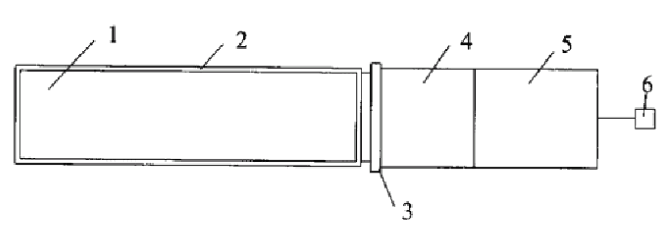
\includegraphics [scale=0.65] {muondensitometer}
  \caption{Датчик мюонного плотномера} 
  \label{img:muondensitometer} 

\end{figure}



В целях снижения временных затрат на измерения с понижением погрешности была предложена конструкция датчика мюонного 
скважинного плотномера (Рис. 1), включающая сцинтилляционный 
детектор (1) с оболочкой (2) и стеклом окна (3), 
фотоумножитель (ФЭУ) (4), усилитель-дискриминатор (5) 
и пульт управления (6).

Физическая длина сцинтилляционного детектора выбирается из 
следующих ограничений. Сцинтилляционная вспышка, 
возникшая на максимальном удалении от фотокатода ФЭУ 
при взаимодействии с мюоном, должна при достижении фотокатода 
иметь достаточно высокий уровень, позволяющий отделить это 
событие от тех сцинтилляционных вспышек, обусловленных 
естественной радиоактивностью исследуемой породы, которые 
возникающих в непосредственной близости от ФЭУ. Это условие 
ограничивают длину сцинтилляционного детектора сверху и 
зависит от коэффициента ослабления света сцинтилляции, 
который для различных сцинтилляционных материалов может 
быть определен расчетом или экспериментально. 

В усилителе-дискриминаторе предусмотрен регулируемый по 
пространственному разрешению плотности порог дискриминации. 
Это позволяет исключить при измерении вклад естественной 
радиоактивности в зависимости от радионуклидов, содержащихся в 
исследуемом грунте, а также регулировать длину рабочего участка 
сцинтилляционного детектора, тем самым настраивая разрешение под 
требования задачи.

В датчике могут быть использованы неорганические, 
органические, пластические и жидкие сцинтилляционные материалы,
что позволяет варьировать как габариты датчика, 
так и его стоимость. 


\begin{figure}[h] 
  \center
  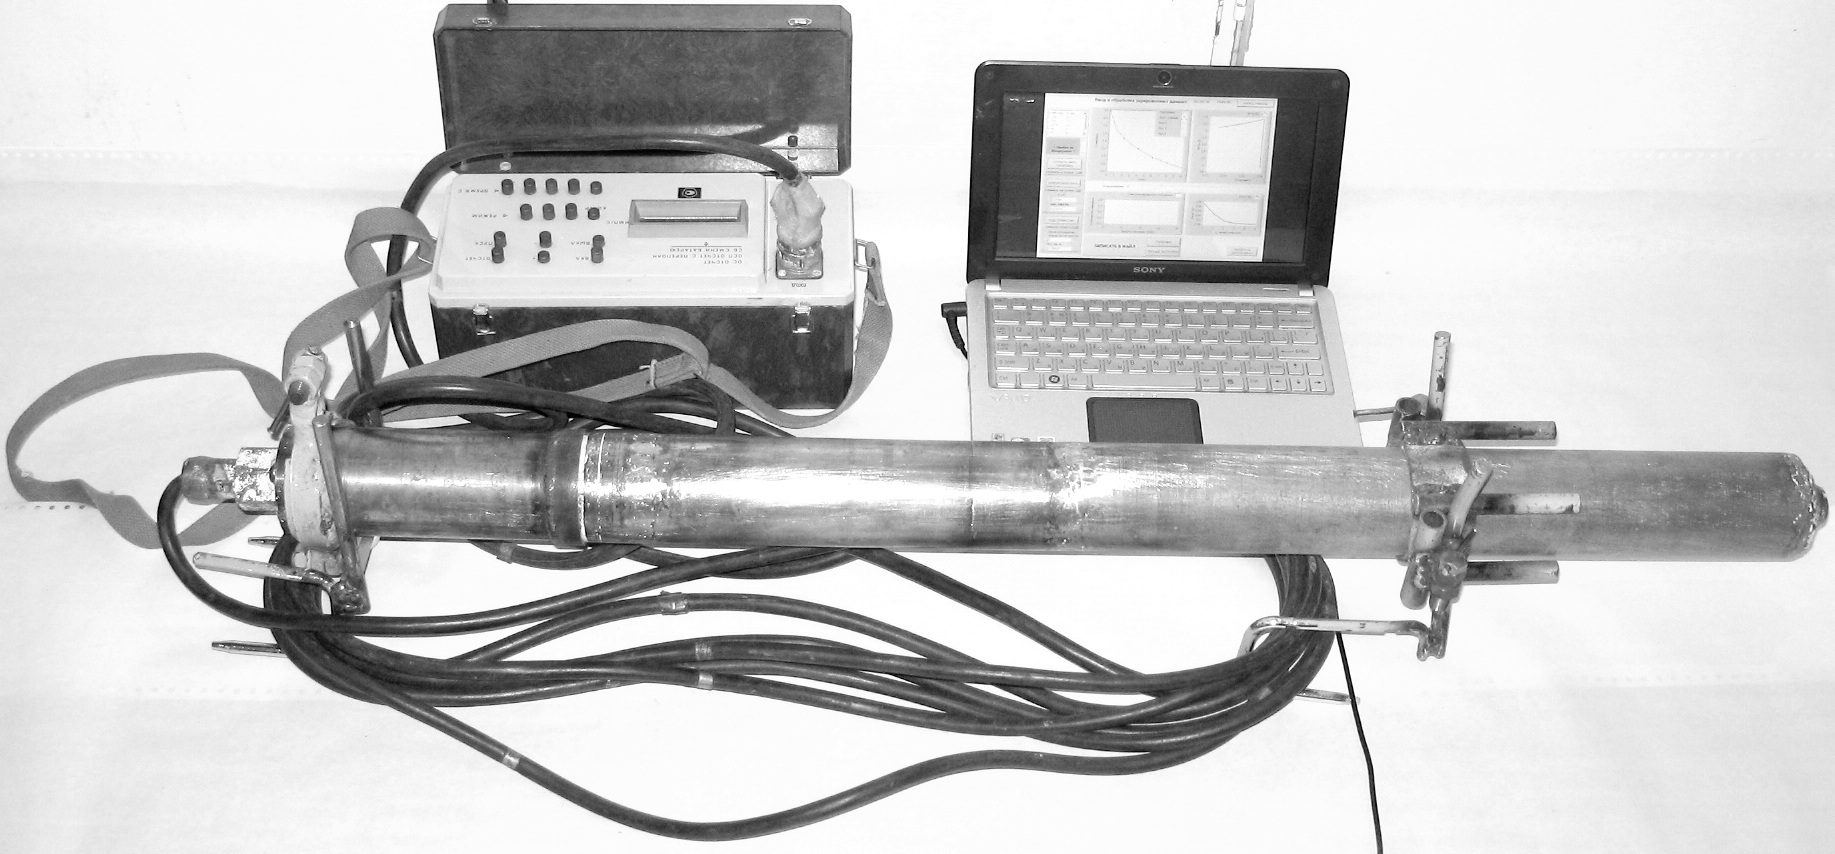
\includegraphics [scale=0.25] {muondensitometer2}
  \caption{Фотография мюонного плотномера} 
  \label{img:muondensitometer2} 

\end{figure}

Предложенная конструкция мюонного скважинного плотномера была 
реализована в пилотном варианте (\ref{img:muondensitometer2}). Плотномер имеет 
герметичный металлический корпус, рассчитанный под диаметр 
обсадной трубы 76 мм. В качестве сцинтилляционного материала 
использован $NaJ(Tl)$. В состав прибора включен 
фотоэлектронный умножитель ФЭУ-93 и  усилитель-дискриминатор, 
выполненный на триггере Шмидта, выход которого согласован с 
блоком управления. Блок управления и регистрации представляет 
собой серийно выпускаемый счетчик импульсов от радиоизотопного 
плотномера ППГР-1. Питание плотномера осуществляется от 
портативного приборного аккумулятора 12 В, 3 А$*$ч. 
Эксплуатационные характеристики макетного варианта 
были опробованы при замере зависимости интенсивности потока 
мюонов от глубины, на воде. 

Резюмируя достоинства мюонного плотномера следует отметить:
\begin{itemize}
  \item Экологическую и биологическую безопасность прибора и 
  связанную с этим простоту эксплуатации при хранении, 
  транспортировке. Отсутствие необходимости в 
  согласованиях его использования с санитарно-эпидемиологическими 
  службами.
  \item Простоту калибровки датчика, не требующей специальных 
  приспособлений. Калибровку проводят в открытых естественных 
  водоемах, на воде – жидкости с низким коэффициентом сжатия. 
  \item Существенное снижение (до двух порядков) объема 
  буровых работ  за счет интегрального характера обследования, 
  значимое особенно в случае дисперсионных грунтов.
  \item Практически приемлемую погрешность (порядка 3\%) и 
  продолжительность измерений (не более 60 минут для глубин до 
  20 м. в. э.).
  \item Компактную конструкцию прибора (длина 0.9 м, масса 7 кг) 
  и простоту его эксплуатации в автономном режиме в течение 8 
  часов непрерывной работы.
\end{itemize}

\clearpage